
\section{Appendix}
\begin{appendices}


\section{Arduino code}
\label{ap:arduino}

In this Section you shall see the Arduino codes that I used inorder to run some components of the DAC system. All the files will be available to you when requested. The following are the codes written for :

\subsection{Motor starting}
{\fontfamily{qcr}\selectfont
\#include<Servo.h> \\
\\
Servo myMotorFL; \\
\\
void setup() \\
\{ \\
 Serial.begin(9600); \\
 myMotorFL.attach(10); \\
 initialize\_motor(); \\
\} \\
\\ 
void initialize\_motor() \\
\{ \\
 Serial.print("Arming the motor!"); \\
 myMotorFL.write(40); //setting low RPM first \\
 delay(1000); \\
\} \\
\\
void loop() \\
\{  \\
  int val = 0;    // setting the motor at 40-130 RPM \\
  Serial.println(millis()); \\        
  myMotorFL.write(val); // letting the motor run at x RPM \\
  delay(1000); \\
\} \\
} \\

\subsection{PID Heater control}
{\fontfamily{qcr}\selectfont
\#include <ZEF.h> \\
ZEF\_ADS ADS;             	    // ADS board for NTC inputs \\
ZEF\_RELAYBOARD  RELAY(8,9);    	    // heater relays \\
ZEF\_PID\_CONTROLLER PID;             // PID heater control: to set PID values, use: ZEF\_PID\_CONTROLLER \\ PID(float Kp, float Ki, float Kd, float controlOutputMin, float controlOutputMax) \\
\\
int WindowSize = 1000;				// logging / control interval in ms \\
unsigned long WindowStartTime; \\
\\
int activeHeater = 0;				// the relay that is currently most active \\
float heaterRatioRelay0\_1 = 3/5;	// The ratio of heat cartridges of relay0 vs the total (relay0 + relay1) \\
float Output = 0; \\
float T\_NTC1, V\_NTC, T\_NTC2; \\
\\
void setup() { \\
\\
    //initialize modules \\
    ADS.begin(); \\
    RELAY.begin(); \\
    PID.begin(); \\
\\
    RELAY.setRelay(0,LOW); // turn relay 0 off \\
    RELAY.setRelay(1,LOW); // turn relay 1 off \\
\\
    Serial.begin(9600); \\
    Serial.setTimeout(50); \\
} \\
\\
void loop() { \\
    // check if window has ended, if so: update sensors, calc new PID output, \& log to serial \\
    if (millis() - WindowStartTime > WindowSize) \\
    { \\
        V\_NTC = ADS.readAbsoluteVoltage(1); \\
        T\_NTC1 = ADS.readNTCTemperature(1); \\
        T\_NTC2 = ADS.readNTCTemperature(2); \\
        Serial.print(millis()); \\
        Serial.print(","); \\
        Serial.print(T\_NTC1,2); \\
        Serial.print(", "); \\
        Serial.print(T\_NTC2,2); \\   
        Serial.println(); \\
\\
        // Calculate Control Output \\
        Output = PID.computeOutput(T\_NTC2); \\
\\
        // set base heater if necessary \\
        if (Output > heaterRatioRelay0\_1) \\
        { \\
            RELAY.setRelay(0,HIGH); \\
            activeHeater = 1; \\
            Output = (Output - heaterRatioRelay0\_1)/(1-heaterRatioRelay0\_1);		// Output adjust for 2nd heater scaling \\
        } \\
        else \\
        { \\
            RELAY.setRelay(1,LOW); \\
            activeHeater = 0; \\
            Output = Output/heaterRatioRelay0\_1;		// Output adjust for 1st heater scaling \\
        } \\
        // Reset window \\
        WindowStartTime = millis(); \\   
    } \\
\\
    // set heaters according to PID output \\
    test = millis()-WindowStartTime; \\
    if (test < Output*WindowSize){RELAY.setRelay(activeHeater,HIGH);} \\
    else {RELAY.setRelay(activeHeater,LOW);} \\
    \\
\\
    // Do communications \\
    checkCommunications(); \\
} \\
\\
void checkCommunications(){ \\
    // see if a command to change the setpoint has been received: \\
    if (Serial.available() > 0){ \\
            byte channel = Serial.read(); \\
            if(channel == 65){          //ASCII value of A \\
            // look for the next valid integer in the incoming serial stream: \\
            int command = Serial.parseFloat(); \\
                if (command>=0){ \\
                float newSetpoint = command; \\
                PID.newSetpoint(newSetpoint); \\
                Serial.print("\# Updated temperature SetPoint for Heaters: "); \\
                Serial.print(newSetpoint); \\
                Serial.println(" deg C"); \\
                } \\
            else{ \\
                Serial.flush(); \\
                Serial.println("\# invalid temperature SetPoint "); \\
                } \\
            } \\
    } \\
}  
}


\newpage
\section{MATLAB code}
\label{ap:MATLAB}

In this Section you shall see the MATLAB codes that I used inorder to evaluate some parameters for the DAC system. All the files will be available to you when requested. The following are the codes written for :

    \subsection{Hole size approximation}
    \label{sec:holesize}

    For calculating the actual hole size of the DAC V2.0 \bigbreak
    
    {\fontfamily{qcr}\selectfont
    
    \%\% Calculating the actual hole size \\

    \% Using paint and for the pixel sizing. \\
    \% I approximately calculated the actual size of the hole. \\
    \% I used a resistor wire which has a dia of 0.445 mm (using a micrometer) as reference \\
    \% Using coordinate geometry and ratios. The distance is calculated as follows. \\

    \%\% For the actual hole size calculation \\
    \%\% 

    \%for the resistor wire \\
    xr1 = 44; \%pixels \\
    yr1 = 63; \%pixels \\
    xr2 = 44; \%pixels \\
    yr2 = 50; \%pixels 
    drs = power((xr2 - xr1), 2) + power((yr2 - yr1), 2); \\
    dr = sqrt(drs); \%pixels \\
    act\_dr = 0.445; \%mm \\
    pix2mm = act\_dr/dr; \%mm/pixels \\

    \%for the resistor wire \\
    xh1 = xr2; \%pixels \\
    yh1 = yr2; \%pixels \\
    xh2 = 45; \%pixels \\
    yh2 = 17; \%pixels \\
    dhs = power((xh2 - xh1),2) + power((yh2 - yh1),2); \\
    dh = sqrt(dhs); \%pixels \\
    act\_dh = act\_dr + (dh*pix2mm); \\

    \%for 0.6mm hole, I am getting 0.9mm approx \\
    \%for 1mm hole, I am getting 1.5mm dia holes approx \\
    }
    
\subsection{Heat exchanger length calculation}


{\fontfamily{qcr}\selectfont
clc; \\
clear; \\

\noindent \%\% Assumptions \\

\noindent \%1. 10  mins to empty it all \\
\% 2. 1 and a half hour to fill 1.5 L \\
\% 3. Density not changing with T \\
\% 4. Cp not changing with T \\
\% 5. Check valve needed at the end, to prevent back flow \\
\% 6. All calculations are done as per - Pg. 62 - 77 for pin fin. \\
\\
\%\% Constants \\
\\
\% For PEI \\
CpPEI = 2000; \%J/kg-K \\
rhoPEI = 1270; \%kg/m3 \\
\\
\% For steel (Swageloke) \\
Ksteel = 502000; \%J/kg-K \\
\\
\% For steel pipe \\
di = 6*E-3; \%m  \\
do = 8*E-3; \%m \\
t = 1*E-3; \%m \\
\\
\% For Fin \\
Dfin = 0.01; \%m \\
lfin = 0.05; \%m \\
\\
\% Natural convection of air \\
h = 8; \%W/m2 - K \\
\\
\%\% Calculation of mass flow \\
\\
\% Assuming that it takes 1 hour to fill 1.5 L of PEI in the system \\
\\
VPEI = 1*E-3; \%m3 \\
tfill = 60*60; \%s \\ 
vdotPEI = VPEI/tfill; \%m3/s \\
mdotPEI = vdotPEI * rhoPEI; \%kg/s \\
\\
\%\% Heat to be removed \\
\\
Tdiff = 120 - 70; \%K, temperature difference between hot PEI and ambient air \\
Qdotremove = mdotPEI*CpPEI*Tdiff; \%W \\
\\
\% \%\% Fin parameters \\
\\
\% Afin = pi*Dfin*lfin; \\
\% Pfin = pi*Dfin; \\
\% beta = sqrt((h*Pfin)/(Ksteel*Afin)); \\
\\
\% \%\% Calculating heat dissipation \\
\\
\% Qdotdiss = Ksteel*Afin*beta*Tdiff*tanh(beta*lfin); \\
\\ 
\% \%\% Calculating number of fins needed \\
\\
\% nfin = Qdotremove/Qdotdiss; \\
\% X = beta*lfin; \\
\% efffin = tanh(X)/(X); \\
\\
\%\% Calculating length of straight finned tube \\
\\
\% Assumptions: \\
\% 1. Getting straight finned tube from Wino's contact \\
\% 2. Using 25.40mm base dia tube (1 inch) \\
\% 3. Using fin height of 9.55mm (the smallest one they have) \\
\% 4. Using fins per meter of 275 (the smallest one they have) \\
\% 5. Assuming fin thickness of 1mm \\
\\ 
\%Area of 1 fin \\
act\_bdia = 25.4*E-3; \%m \\
act\_hfin = 15.8*E-3; \%m \\
term1 = power((act\_bdia + act\_hfin),2); \\
term2 = power((act\_bdia - act\_hfin),2); \\
act\_Afin = 2*pi*(term1 - term2)/4; \%m2 \\
nfinperm = 275; \%no. of fins per m \\
\\
\%Heat dissipated from 1 fin \\
act\_Qdis = h*act\_Afin*Tdiff; \%W \\
\\
\%No. of fins needed for the complete heat dissipation \\
act\_nfin = Qdotremove/ac\_Qdis; \%no. of fins \\
\\
\%Length of the straight finned tube needed \\
act\_lfin = act\_nfin*100/nfinperm; \%cm \\
}



\newpage
\section{Fusion 360 drawings}
\label{ap:fusion}

\subsection{DAC V1.1 System}

\subsubsection{Distributor}

\begin{figure}[H]
    \centering
    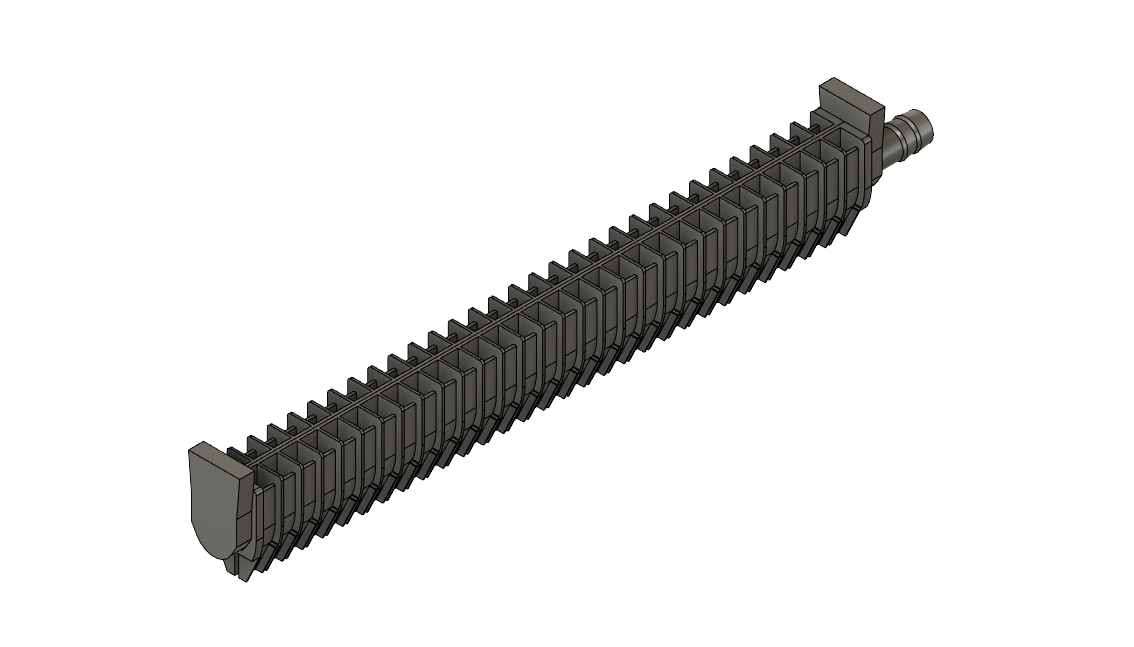
\includegraphics[scale = 0.4]{images/mywork/Sprint4/Distributor_old.png}
    \caption{DAC V1.1 Distributor}
    \label{fig:dacv1.1dis}
\end{figure}


\subsubsection{Manifold}

\begin{figure}[H]
    \centering
    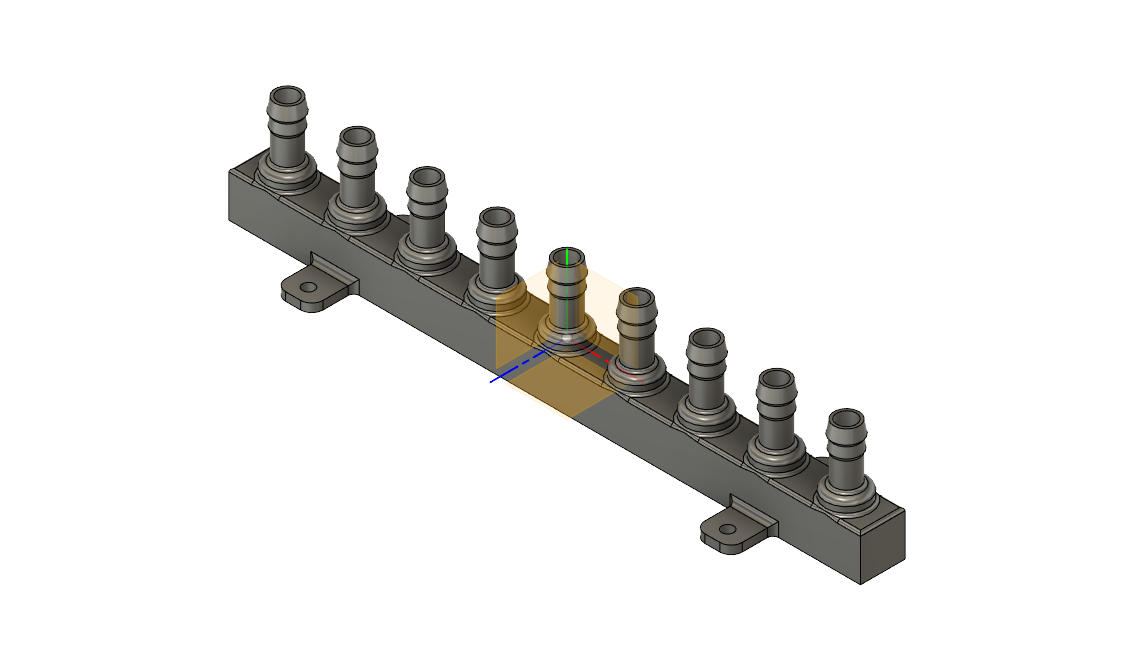
\includegraphics[scale = 0.4]{images/mywork/Sprint4/Manifold_old.png}
    \caption{DAC V1.1 Manifold}
    \label{fig:dacv1.1mani}
\end{figure}


\subsubsection{Collector}

\begin{figure}[H]
    \centering
    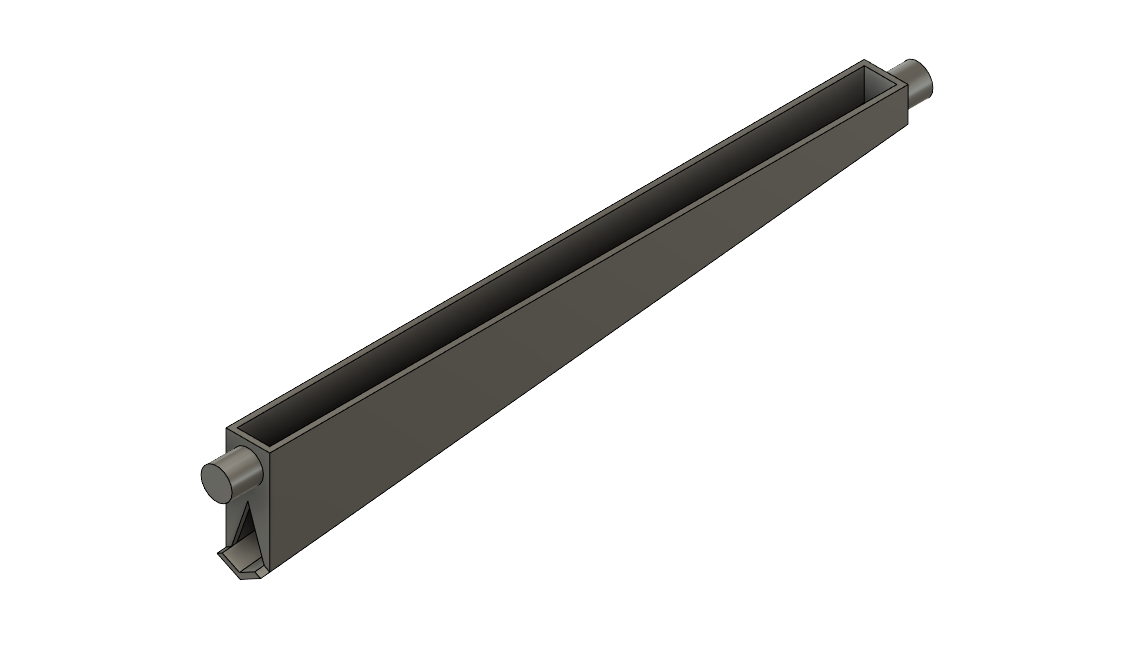
\includegraphics[scale = 0.4]{images/mywork/Sprint4/Collector_old.png}
    \caption{DAC V1.1 Collector}
    \label{fig:dacv1.1coll}
\end{figure}

\subsubsection{Collector bucket}

\begin{figure}[H]
    \centering
    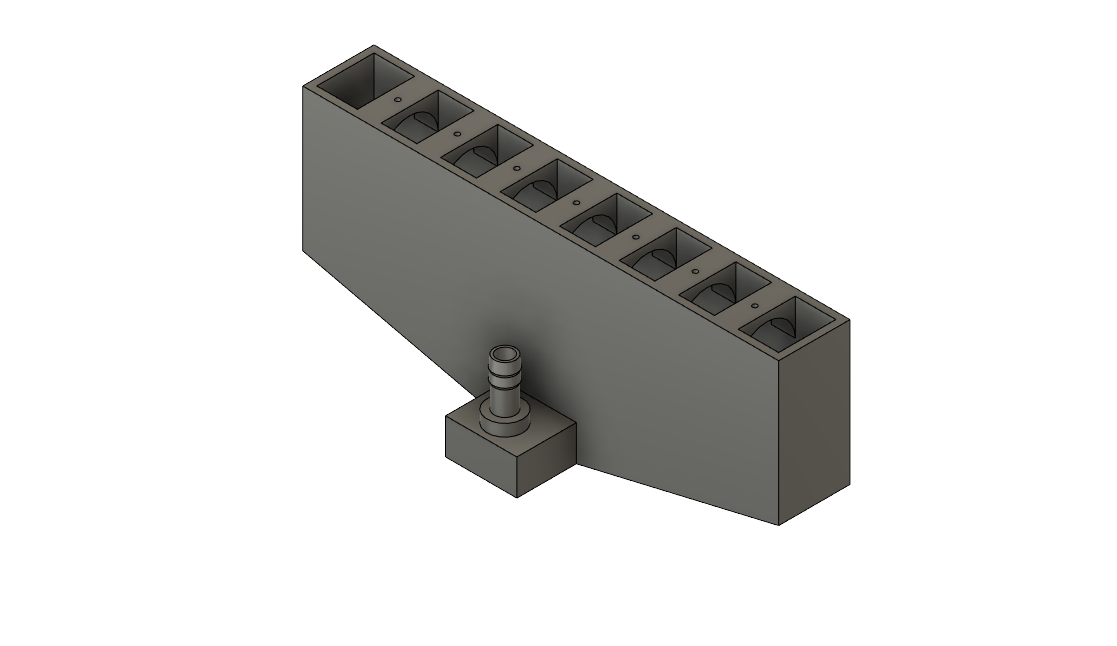
\includegraphics[scale = 0.4]{images/mywork/Sprint4/DACcollbuc_old.png}
    \caption{DAC V1.1 Collector bucket}
    \label{fig:dacv1.1collbuc}
\end{figure}



\subsection{DAC V2.0 System}

\subsubsection{Distributor}

\begin{figure}[H]
    \centering
    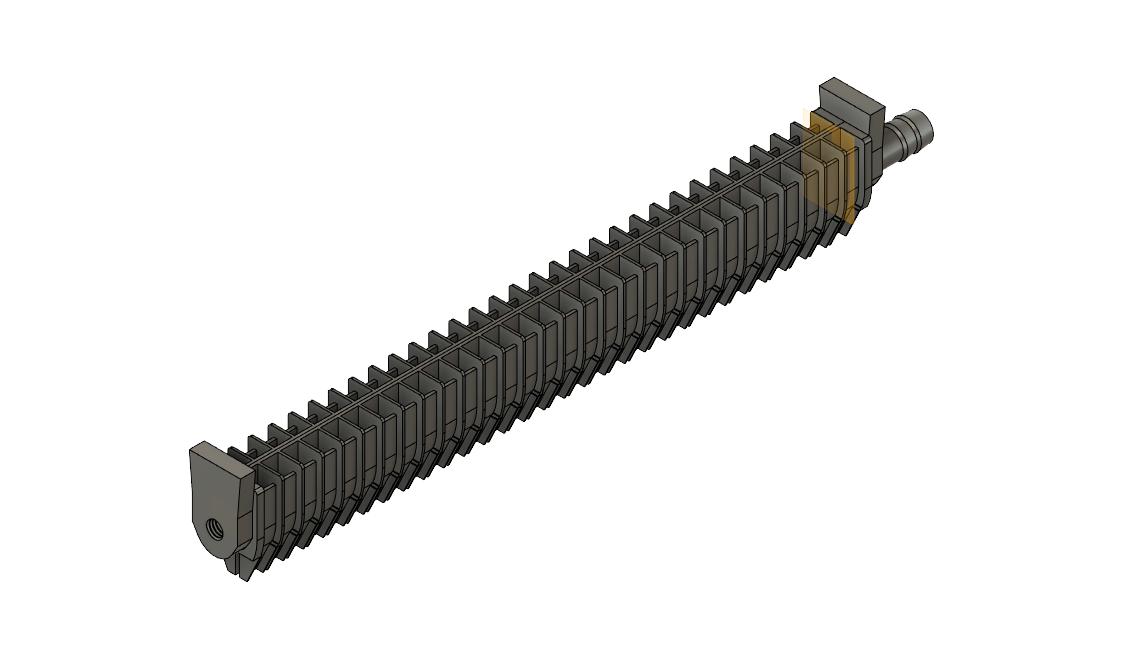
\includegraphics[scale = 0.4]{images/mywork/Sprint4/Distributor_main.png}
    \caption{DAC V2.0 Distributor}
    \label{fig:dacv2dis}
\end{figure}



\subsubsection{Manifold}

\begin{figure}[H]
    \centering
    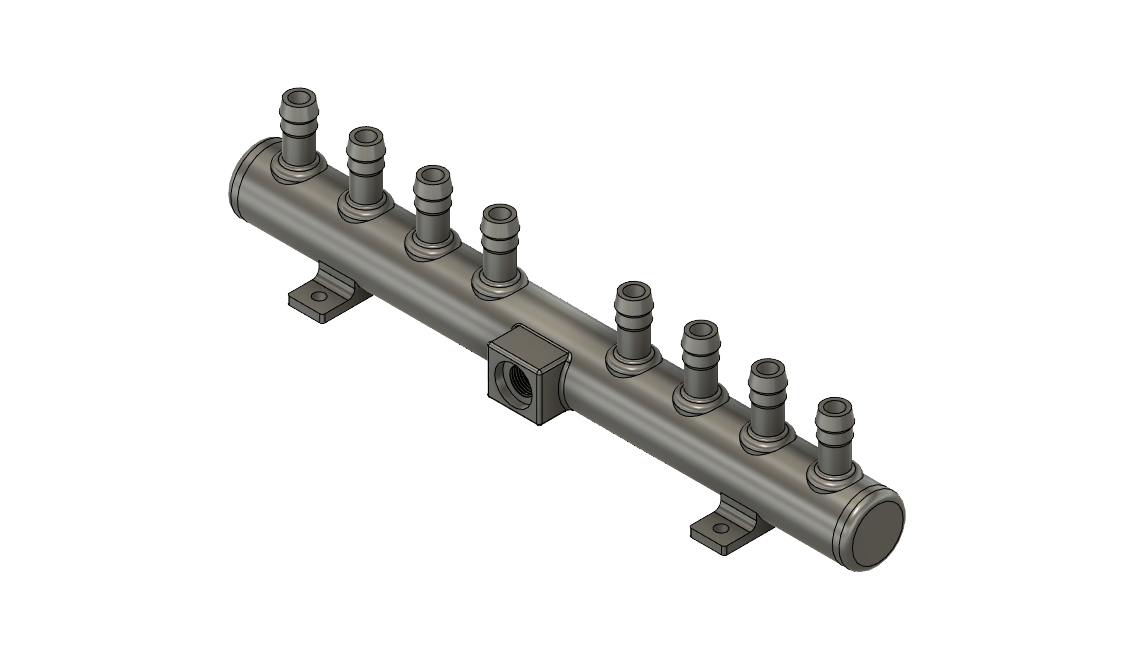
\includegraphics[scale = 0.4]{images/mywork/Sprint4/Manifold_main.png}
    \caption{DAC V2.0 Manifold}
    \label{fig:dacv2mani}
\end{figure}


\subsubsection{Collector}

\begin{figure}[H]
    \centering
    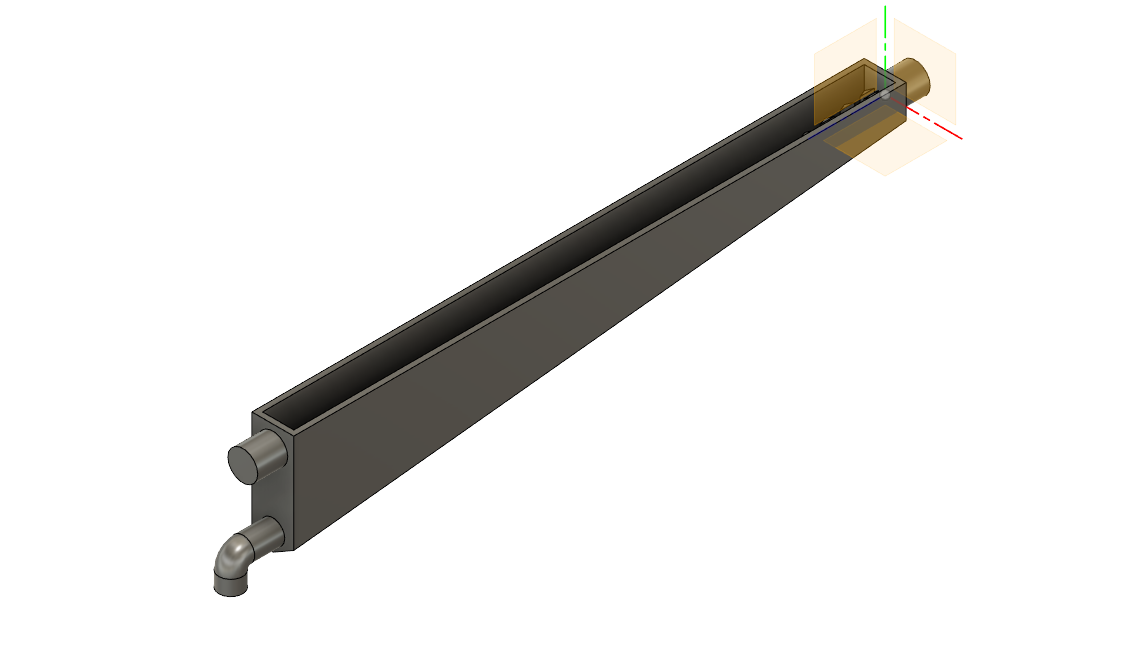
\includegraphics[scale = 0.4]{images/mywork/Sprint4/Collector_main.png}
    \caption{DAC V2.0 Collector}
    \label{fig:dacv2coll}
\end{figure}


\subsubsection{Collector bucket}

\begin{figure}[H]
    \centering
    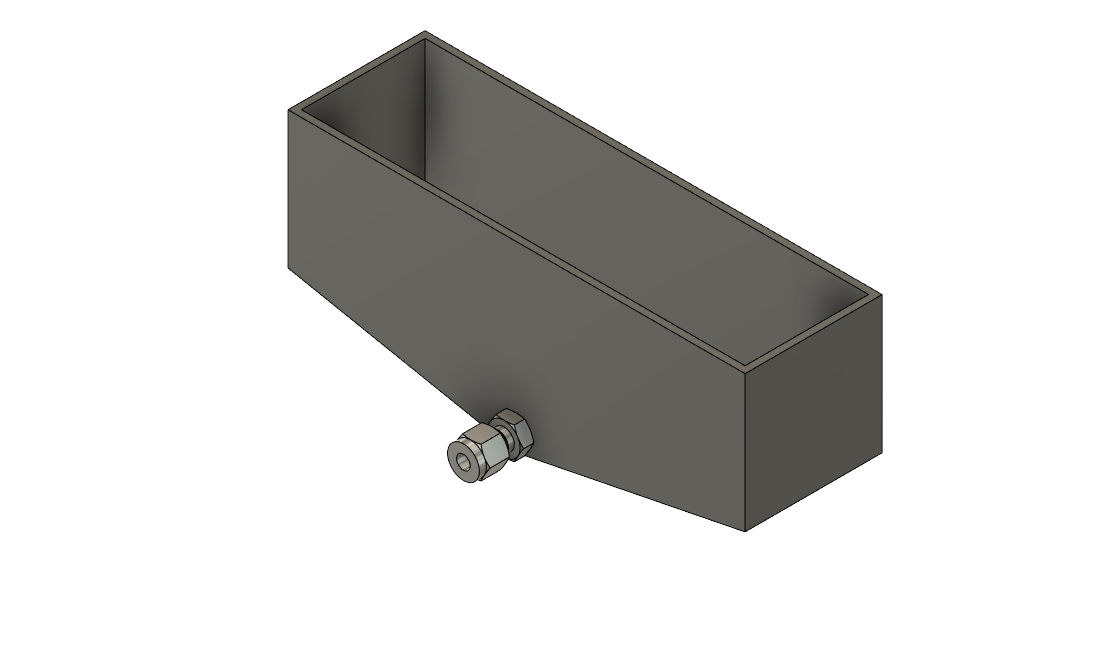
\includegraphics[scale = 0.4]{images/mywork/Sprint4/DACcollbuc_new.png}
    \caption{DAC V2.0 Collector bucket}
    \label{fig:dacv2collbuc}
\end{figure}


\subsection{The set - up}

\begin{figure}[H]
    \centering
    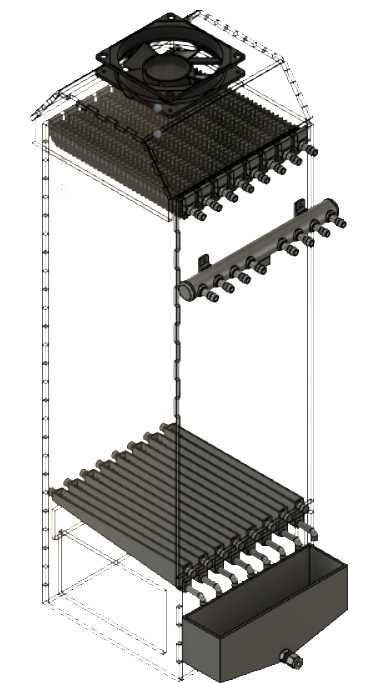
\includegraphics[scale = 1.4]{images/mywork/Sprint4/DACV2Absorber.png}
    \caption{DAC V2.0 Absorber}
    \label{fig:dacv2abs}
\end{figure}

\subsection{The complete set - up}
\label{sec:setup2.0}

\begin{figure}[H]
    \centering
    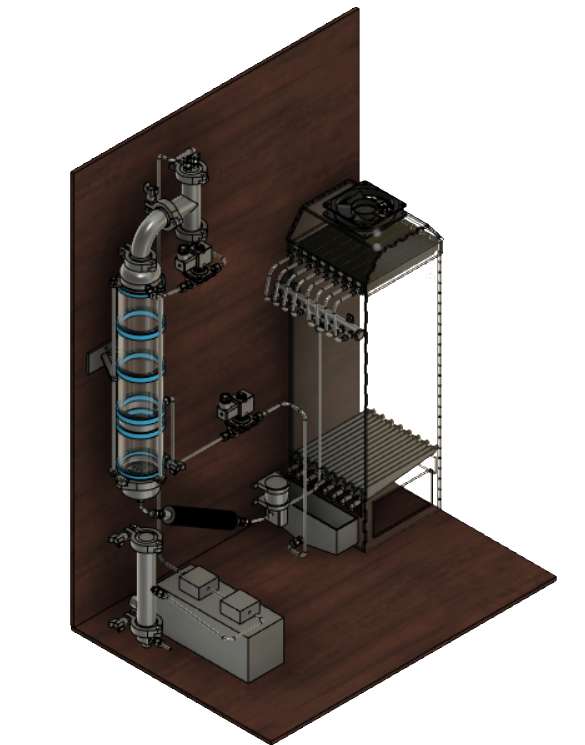
\includegraphics[scale = 1.4]{images/mywork/Sprint4/DACV2system1.png}
    \caption{DAC V2.0 System}
    \label{fig:dacv2system}
\end{figure}





\end{appendices}
